\chapter{Relato de Experiência}
\label{cap:relato}

\section{Contextualização do Projeto}

O Sistema Integrado de Processos Seletivos (SIPROS) é uma plataforma institucional da Universidade Federal de Goiás (UFG), projetada para centralizar a criação e o acompanhamento de editais. A criticidade desse sistema é alta, uma vez que ele transaciona dados sensíveis de candidatos e gerencia documentos oficiais da instituição.

No momento em que o projeto foi assumido pela equipe, o software encontrava-se em uma fase de desenvolvimento na qual a arquitetura de segurança e a integração de componentes estavam em transição. Para fins de prototipação inicial, o sistema utilizava credenciais inseridas provisoriamente no código (\textit{hardcoded}), a comunicação entre o \textit{front-end} e o \textit{back-end} ainda necessitava de consolidação estrutural, e alguns fluxos de acesso eram simulados (\textit{mocks}). O principal objetivo do projeto neste semestre consistiu em evoluir essa base arquitetural, substituindo as abordagens provisórias por implementações definitivas e estabelecendo um fluxo de autenticação robusto.

\subsection{Ambiente Organizacional}

O relato ocorreu no contexto da disciplina de Prática em Engenharia de Software (Fábrica de Software), cujo objetivo é proporcionar vivência realista na manutenção e evolução de um sistema de grande porte. A equipe responsável, denominada "Equipe Dourada", foi composta por sete discentes. Destes, Ester e Lucas atuaram predominantemente na comunicação técnica com a coordenação, que por sua vez assumiu o papel semelhante ao de um \textit{Product Owner} (PO).

Para o gerenciamento do processo de desenvolvimento, a equipe optou por uma metodologia flexível inspirada no \textit{Scrum} e no \textit{Kanban}. O trabalho foi organizado em iterações regulares (\textit{Sprints}) de duas semanas, ao fim das quais ocorriam reuniões de revisão diretamente com a coordenação para a validação das entregas. As principais tecnologias e ferramentas empregadas englobaram o Angular para o \textit{front-end}, Keycloak para o gerenciamento de identidades, Docker para o encapsulamento do ambiente, Figma para o \textit{design} de interfaces e a plataforma GitHub para versionamento de código e gestão das tarefas. Uma representação visual de como as tarefas eram distribuídas e acompanhadas através do quadro Kanban no GitHub Projects pode ser vista na Figura \ref{fig:kanban}.

\begin{figure}[H]
 \centering
 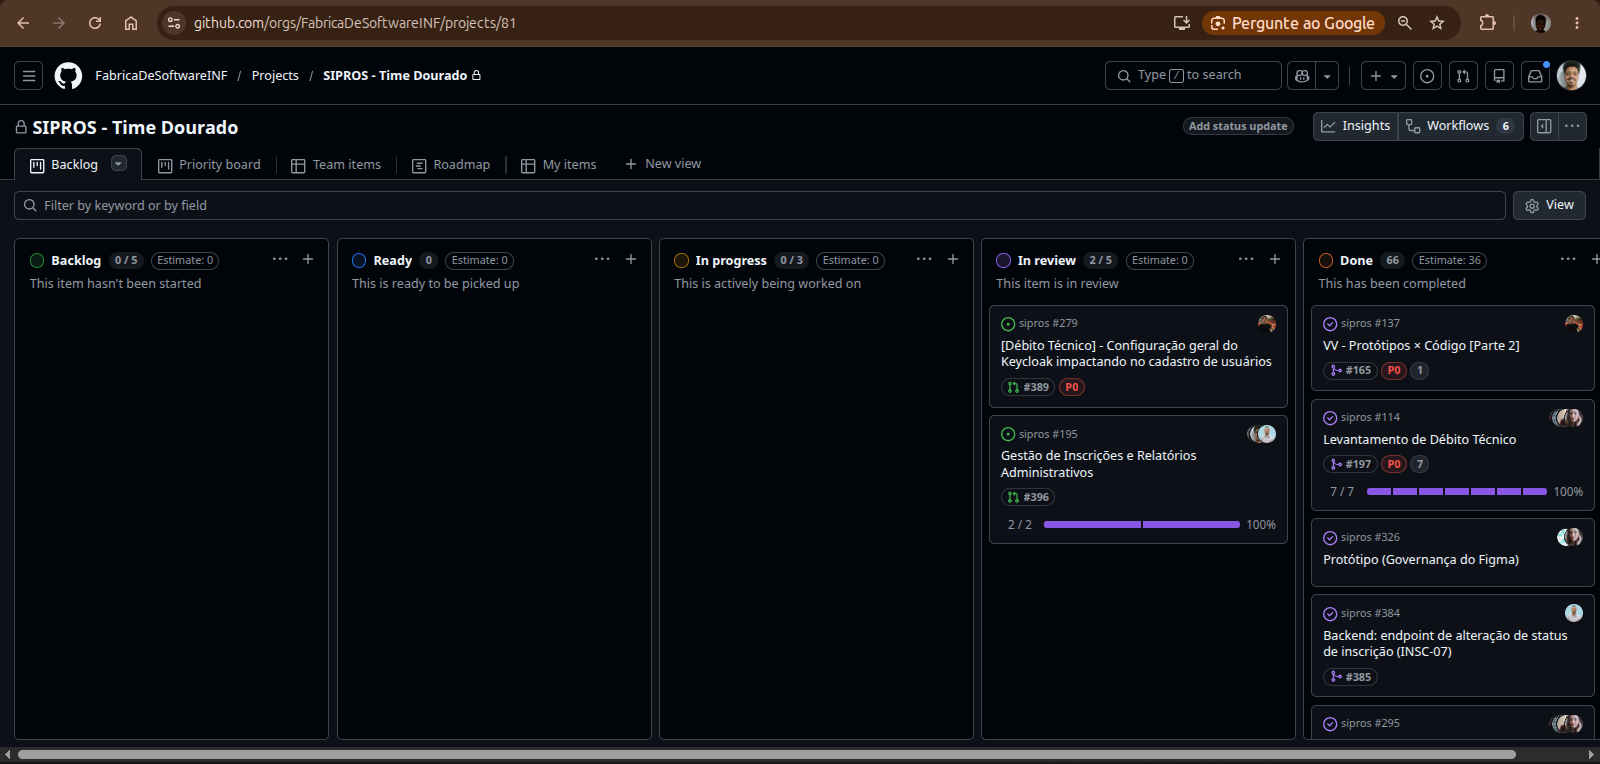
\includegraphics[width=0.9\textwidth]{./fig/fluxo_trabalho_kanban.png}
 \caption{Quadro Kanban utilizado para o acompanhamento e gestão das tarefas da equipe.}
 \label{fig:kanban}
\end{figure}

\subsection{Forma de Participação no Projeto}

O autor do trabalho ingressou no projeto exercendo o papel de desenvolvedor \textit{full-stack}. A integração ao ambiente tecnológico ocorreu por meio de um \textit{onboarding} estruturado pela própria Fábrica, cujo foco foi o nivelamento prático em controle de versão no Git e na orquestração de contêineres via Docker. Essa familiarização inicial garantiu que todo o ambiente de desenvolvimento local operasse de maneira isolada e padronizada, permitindo uma transição fluida para as atividades de codificação do sistema legado.

\section{Atividades Realizadas e Resultados Gerados}

As atividades desenvolvidas abrangeram a intervenção simultânea em três frentes principais: segurança, interface e testes automatizados. A seguir, detalham-se as principais contribuições técnicas executadas pelo autor.

A primeira frente consistiu na refatoração da camada de segurança (\textit{Issue} \#214 e \#253). O desenvolvimento exigiu a substituição do fluxo estático pela integração com o protocolo OAuth 2.0 via Keycloak, empregando especificamente o fluxo \textit{Authorization Code} acoplado à extensão PKCE. A adoção desse padrão mitigou os riscos inerentes a aplicações de página única (SPA), protegendo o processo de delegação de acesso contra a interceptação de \textit{tokens}. Adicionalmente, implementou-se o redirecionamento automático para a autenticação centralizada do Google, otimizando a experiência do usuário final.

A segunda frente pautou-se nos processos de Verificação e Validação de interface (\textit{Issue} \#139 e \#179). A atividade focou no levantamento de divergências estruturais entre a documentação oficial (Casos de Uso) e os protótipos de alta fidelidade desenhados no Figma, resultando em correções aplicadas diretamente nos componentes visuais desenvolvidos em Angular.

A terceira frente atuou na Garantia da Qualidade (QA). O autor estruturou o ambiente básico da suíte de testes de unidade (\textit{Issue} \#304). O propósito dessa implementação foi prevenir que as refatorações arquiteturais resultassem em regressões nas regras de negócio da aplicação.

\section{Integração com a Equipe e Processo de Trabalho}

A dinâmica de trabalho colaborativo pautou-se na autonomia técnica e na comunicação proativa. Os alinhamentos diários ou de acompanhamento foram centralizados no Discord (ferramenta oficial para chamadas de voz e revisões conjuntas) e em grupos no WhatsApp (para comunicação ágil). 

O processo de trabalho da equipe exigiu um gerenciamento cuidadoso para lidar com conflitos de código. Essa coordenação foi feita estabelecendo a clareza sobre qual ramificação (\textit{branch}) cada desenvolvedor possuía responsabilidade em dado momento, mitigando sobreposições no repositório. O processo exigia, por definição, que qualquer alteração proposta (\textit{Pull Request}) passasse pelo fluxo estruturado de revisão antes de ser integrada à aplicação principal.

\section{Desafios Enfrentados}

Os desafios apresentados possuíram naturezas tanto técnicas quanto de engenharia de requisitos. Do ponto de vista técnico, o \textit{onboarding} na configuração do Keycloak exigiu aprendizado sobre os escopos e as diretrizes do \textit{Google Cloud Platform} (GCP). Houve também complexidade substancial na manutenção dos estados do aplicativo Angular, devido à perda de contexto gerada pelos redirecionamentos inerentes ao fluxo de autenticação externo.

Quanto aos desafios organizacionais, a principal dificuldade encontrada referiu-se à inexistência de uma "fonte da verdade" unificada. Os desenvolvedores debatiam-se constantemente frente à contradição entre os requisitos técnicos descritos nos modelos textuais de Casos de Uso e o que estava desenhado nos protótipos visuais no Figma.

\section{Soluções Adotadas e Resultados Obtidos}

Para solucionar os impasses organizacionais relativos aos requisitos, a equipe deliberou e oficializou que os documentos de Casos de Uso funcionariam como a única fonte da verdade em caso de divergência com os protótipos visuais. 

No âmbito técnico, a substituição definitiva das telas estáticas e da autenticação em \textit{mock} pela implementação do fluxo OAuth/PKCE trouxe maturidade ao sistema. A aplicação das correções de V\&V erradicou diversas inconsistências visuais, e a infraestrutura do repositório foi higienizada com a migração das credenciais embutidas no código para variáveis de ambiente isoladas. Como resultado prático consolidado, o SIPROS evoluiu de um estado acadêmico experimental para uma arquitetura de \textit{software} aderente às diretrizes de segurança de mercado.

\section{Avaliação de Qualidade de Software}

A estratégia de qualidade ancorou-se em dois eixos paralelos de validação. O primeiro envolveu a estruturação de uma fundação formal para testes de unidade automatizados voltados ao \textit{back-end}, provendo a segurança indispensável para a evolução orgânica do código. O segundo eixo foi ancorado fortemente no fator humano por meio do processo obrigatório de \textit{Code Review}. Estabeleceu-se como norma inegociável que nenhuma alteração técnica seria introduzida na ramificação principal sem o escrutínio e aprovação por pares, assegurando aderência aos padrões de código preestabelecidos. A Figura \ref{fig:code_review} exemplifica a aplicação desta prática, evidenciando o painel de aprovação de um \textit{Pull Request} que passou pelo crivo da equipe.

\begin{figure}[H]
 \centering
 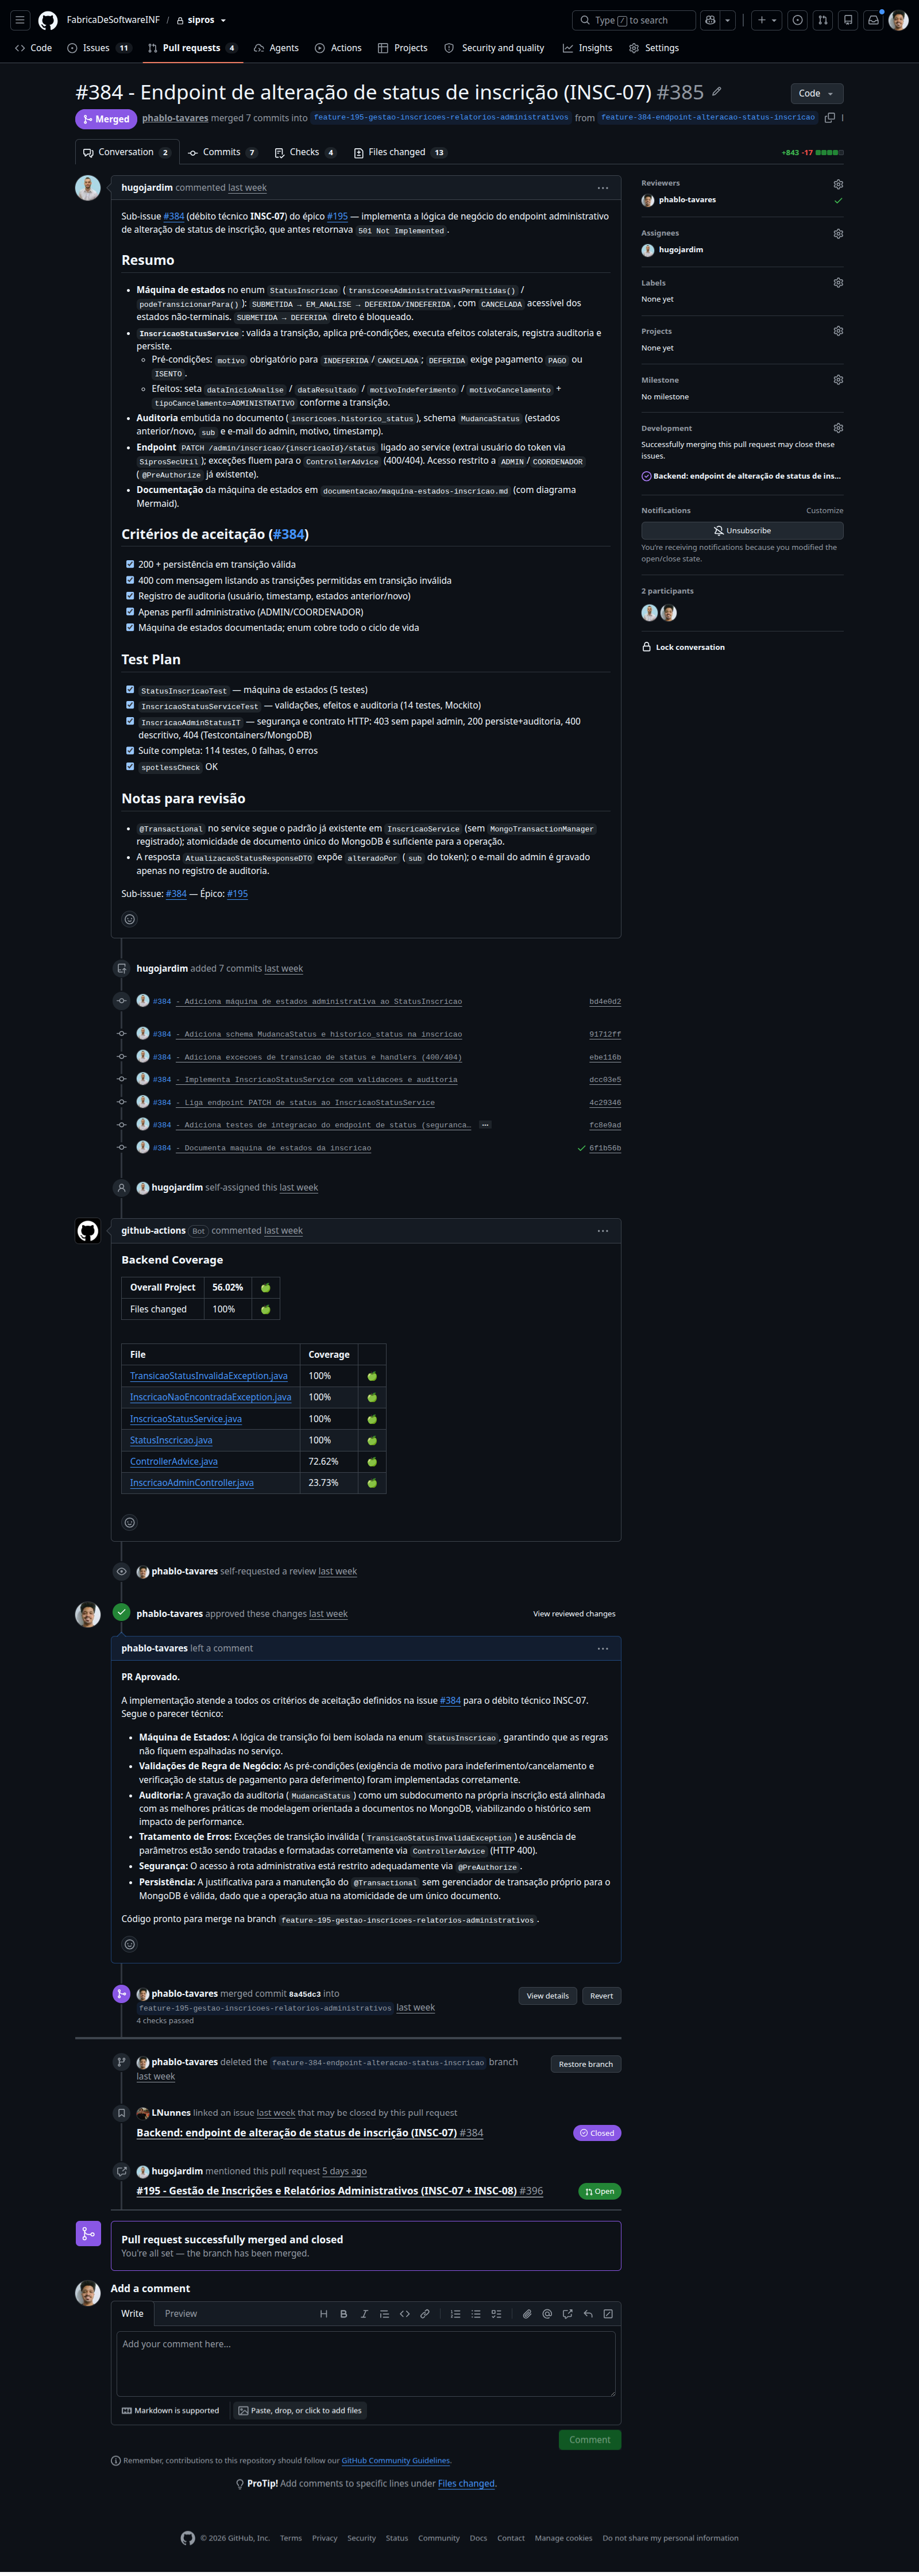
\includegraphics[width=0.9\textwidth]{./fig/evidencia_code_review.png}
 \caption{Evidência do processo de \textit{Code Review} exigido antes da integração de novas funcionalidades.}
 \label{fig:code_review}
\end{figure}

\section{Aprendizados e Desenvolvimento Profissional}

A vivência na Fábrica de Software extrapolou o aprendizado estritamente acadêmico ao submeter o autor a responsabilidades genuínas exigidas pelo mercado de trabalho. No espectro das \textit{hard skills}, a experiência solidificou o domínio de protocolos modernos de autenticação (GCP, Keycloak, OAuth 2.0), além da consolidação prática no desenvolvimento voltado para o ecossistema Angular e na orquestração de contêineres Docker.

No tocante às \textit{soft skills}, houve uma evolução marcante na capacidade de autogerenciamento, na resolução autônoma de bloqueios operacionais e na proficiência em debater arquitetura técnica com outros profissionais. Ao final do projeto, o discente consolidou a visão de que atuar na manutenção e refatoração crítica de uma aplicação preexistente confere um peso e um realismo profissional incomensuráveis, complementando sua formação integral como Engenheiro de Software.
